\documentclass[11pt,a4paper]{article}
\usepackage[utf8]{inputenc}
\usepackage[spanish]{babel}
\usepackage{amsmath}
\usepackage{amsfonts}
\usepackage{amssymb}
\usepackage{float}
\usepackage{graphicx}
\usepackage[left=2cm,right=2cm,top=2cm,bottom=2cm]{geometry}
\usepackage{caption}
\captionsetup[table]{name=Tabla}
\author{Marina Esgueva Ruiz}
\title{Comparación centros}
\begin{document}
\begin{table}
\caption{Error cuadrático medio. EDP 1.}
\centering
\begin{tabular}{|c|cc|cc|}
\hline
\   & \multicolumn{2}{c|}{Diferencias en la frontera} & \multicolumn{2}{c|}{Error en la frontera} \\
\hline
\ N & $\epsilon$ fijo & $\epsilon$ variable & $\epsilon$ fijo & $\epsilon$ variable \\
\hline
\ 20 & 3.7211e-03&  2.5625e-03 & 3.7211e-03 & 3.1905e-03 \\
\ 25 &  9.9508e-05 & 9.8904e-04& 9.6414e-05 & 1.0571e-03 \\
\ 30 &  6.3017e-04 &6.8460e-04 & 5.8700e-05 & 1.0768e-03\\
\ 35 & 2.6278e-05 & 5.0020e-04 & 4.5834e-05&  4.3269e-05 \\
\ 40& 8.7509e-06 &4.6296e-05& 1.5622e-05 &9.5770e-06\\
\ 50& 3.1006e-06& 8.6069e-06 & 2.3243e-06 &  2.4942e-06\\
\hline
\end{tabular}
\end{table}
\begin{figure}

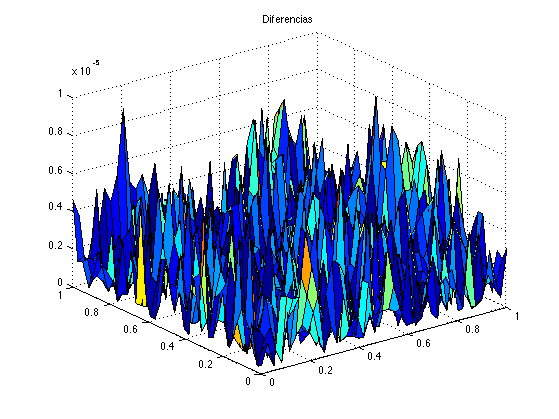
\includegraphics[scale=.27]{diferencias1.png}
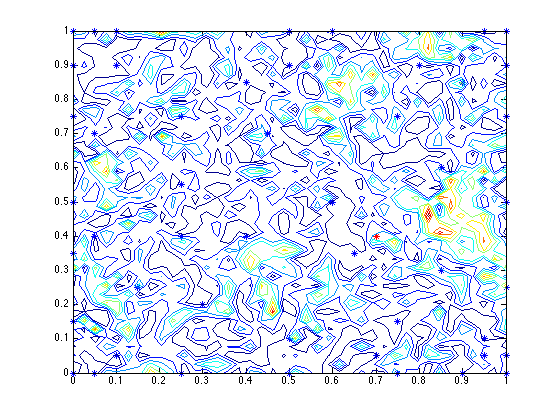
\includegraphics[scale=.27]{centros1.png}
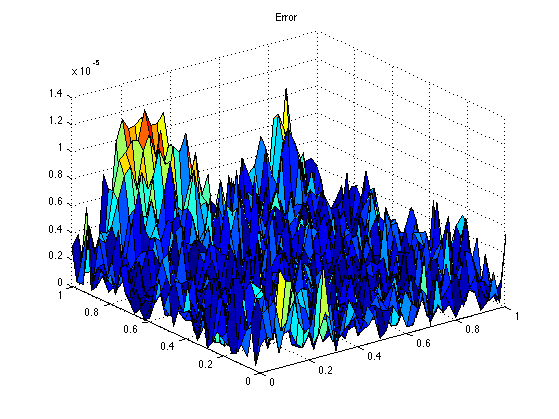
\includegraphics[scale=.27]{error1.png}
\caption{Diferencia entre soluciones en la frontera. Parámetro fijo}
\end{figure}

\begin{figure}

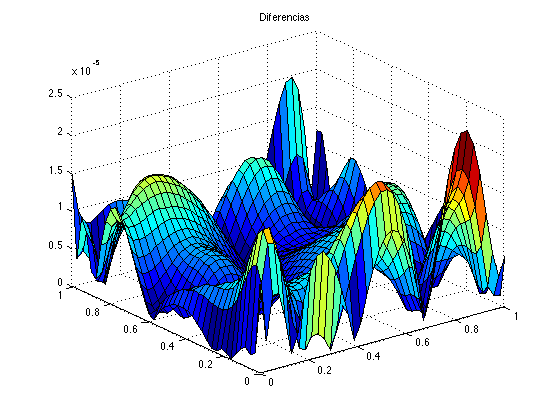
\includegraphics[scale=.27]{diferencias2.png}
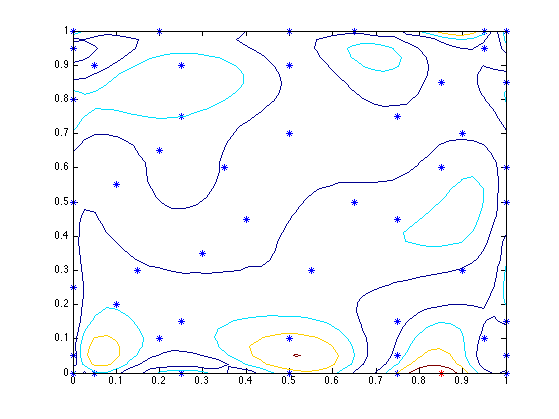
\includegraphics[scale=.27]{centros2.png}
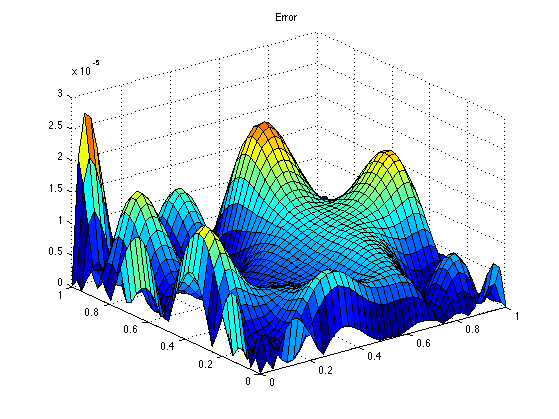
\includegraphics[scale=.27]{error2.png}
\caption{Diferencia entre soluciones en la frontera. Parámetro variable}
\end{figure}

\begin{figure}

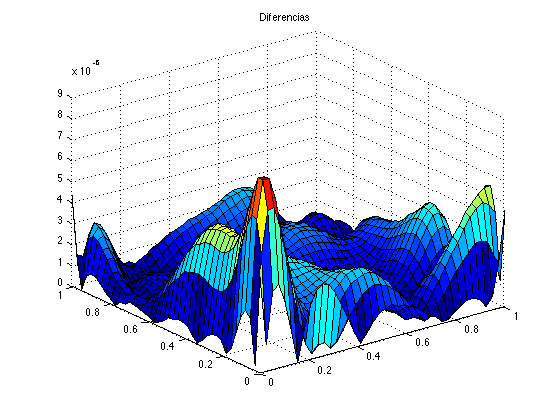
\includegraphics[scale=.27]{diferencias3.png}
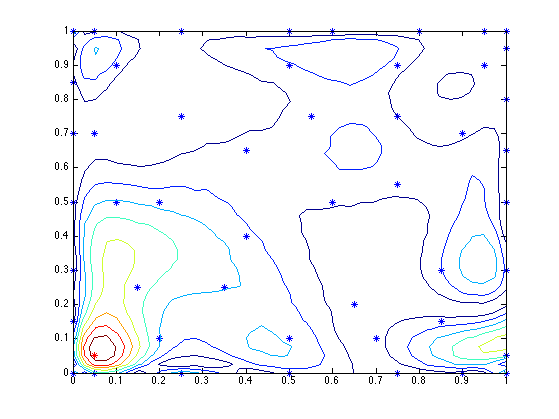
\includegraphics[scale=.27]{centros3.png}
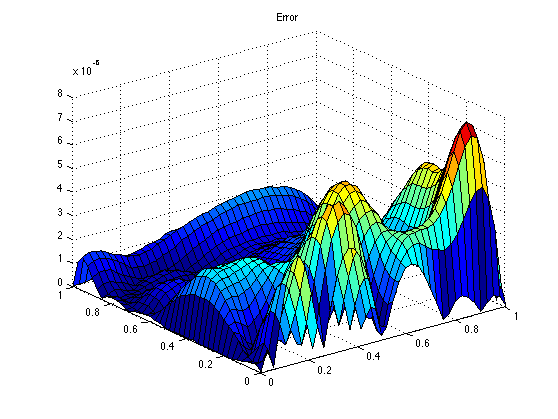
\includegraphics[scale=.27]{error3.png}
\caption{Error en la frontera. Parámetro fijo}
\end{figure}


\begin{figure}

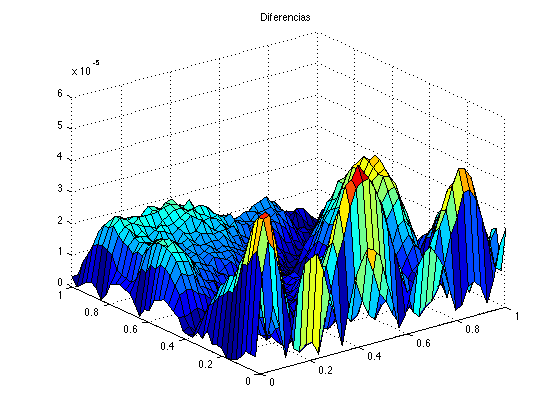
\includegraphics[scale=.27]{diferencias4.png}
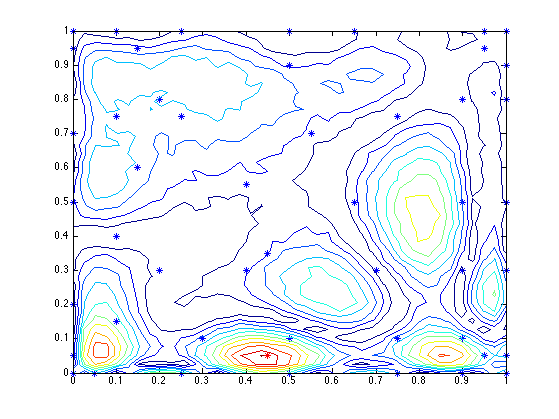
\includegraphics[scale=.27]{centros4.png}
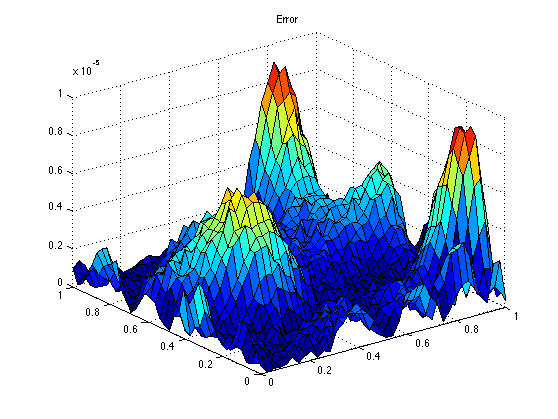
\includegraphics[scale=.27]{error4.png}
\caption{Error en la frontera. Parámetro variable}
\end{figure}
\begin{table}
\caption{Error cuadrático medio. EDP 3.}
\centering
\begin{tabular}{|c|cc|cc|}
\hline
\   & \multicolumn{2}{c|}{Diferencias en la frontera} & \multicolumn{2}{c|}{Error en la frontera} \\
\hline
\ N & $\epsilon$ fijo & $\epsilon$ variable & $\epsilon$ fijo & $\epsilon$ variable \\
\hline
\ 20 & 6.7488e-02 & 1.1757e-02 & 4.5215e-03& 1.2365e-01 \\
\ 25 & 5.1936e-03& 4.7884e-03&  5.8204e-02&  9.4766e-03\\
 \ 30 & 1.6244e-03& 4.1728e-03& 6.8239e-04 & 2.0990e-03 \\
 \ 35 &2.8328e-04& 6.5872e-04 &  1.0899e-03& 8.7842e-04 \\
 \ 40  & 2.3212e-04& 1.7510e-04 & 4.4141e-04 & 2.0527e-04 \\
 \ 50 &  7.8318e-05& 1.8564e-04 &7.5225e-04 & 4.2525e-05\\
 \hline
 \end{tabular}
 \end{table}
 
 \begin{figure}

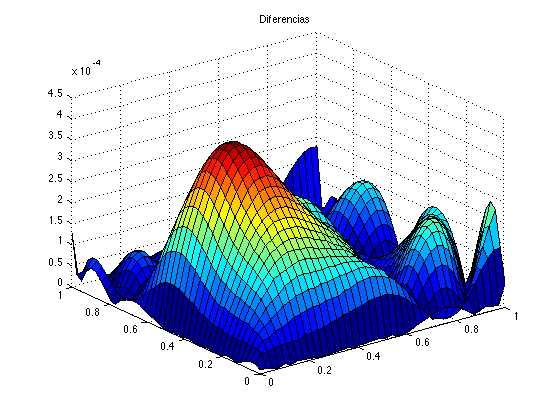
\includegraphics[scale=.27]{diferencias1_3.png}
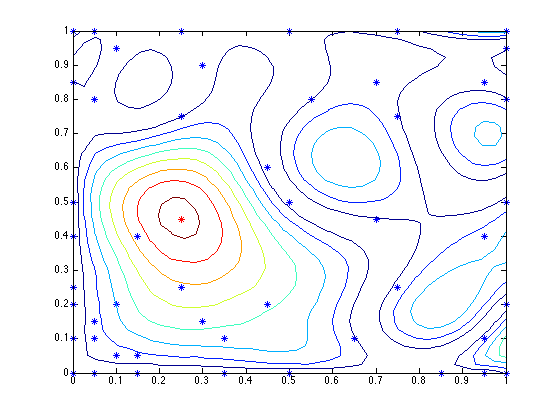
\includegraphics[scale=.27]{centros1_3.png}
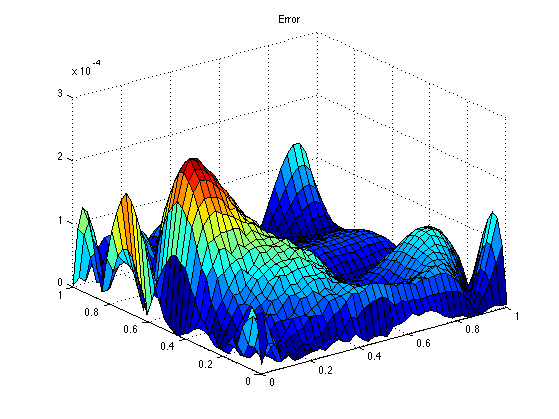
\includegraphics[scale=.27]{error1_3.png}
\caption{Diferencia entre soluciones en la frontera. Parámetro fijo}
\end{figure}

\begin{figure}

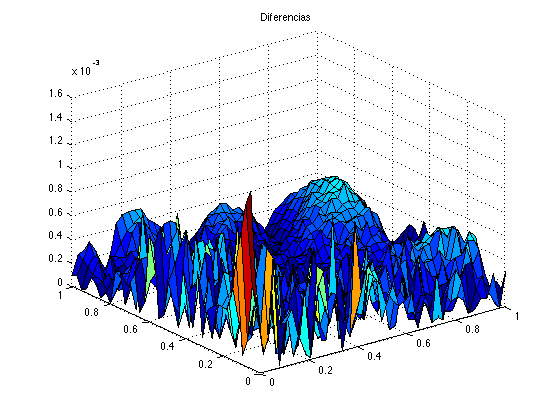
\includegraphics[scale=.27]{diferencias2_3.png}
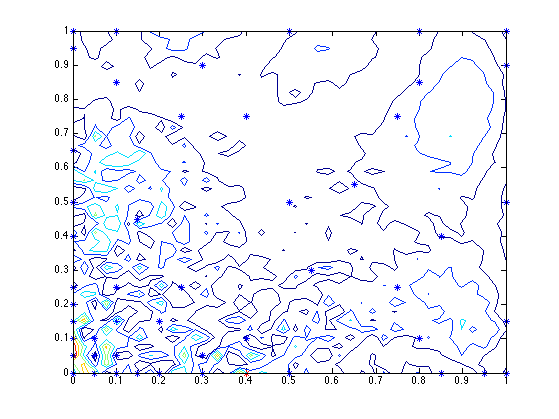
\includegraphics[scale=.27]{centros2_3.png}
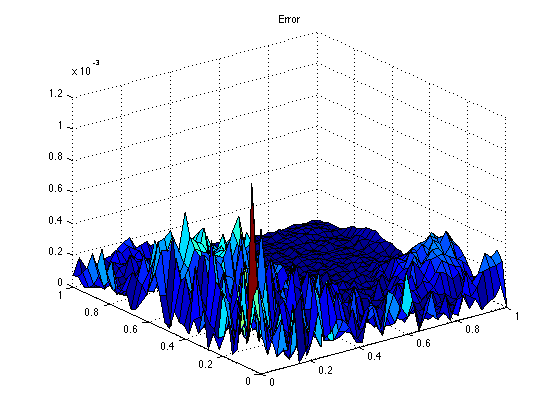
\includegraphics[scale=.27]{error2_3.png}
\caption{Diferencia entre soluciones en la frontera. Parámetro variable}
\end{figure}

\begin{figure}

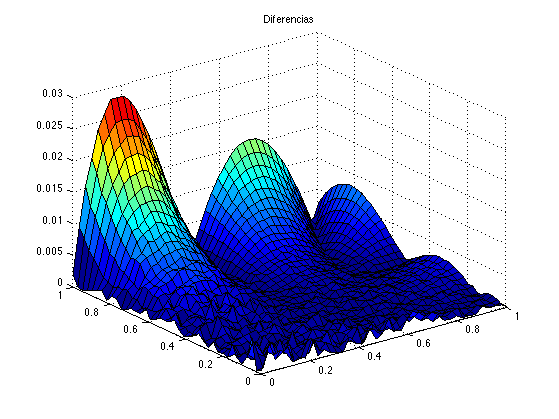
\includegraphics[scale=.27]{diferencias3_3.png}
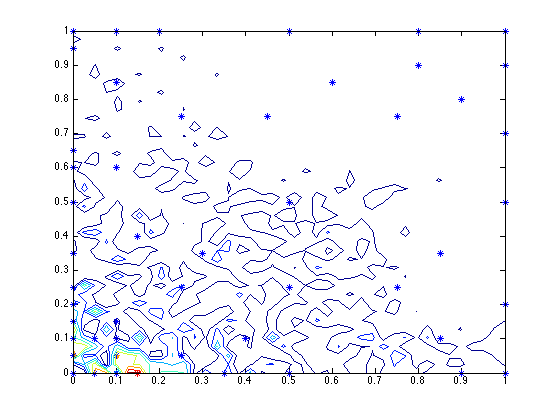
\includegraphics[scale=.27]{centros3_3.png}
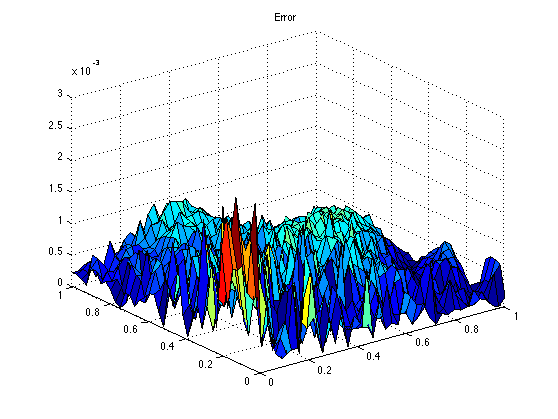
\includegraphics[scale=.27]{error3_3.png}
\caption{Error en la frontera. Parámetro fijo}
\end{figure}


\begin{figure}

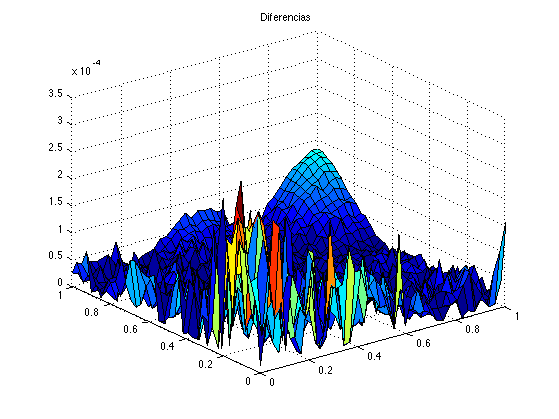
\includegraphics[scale=.27]{diferencias4_3.png}
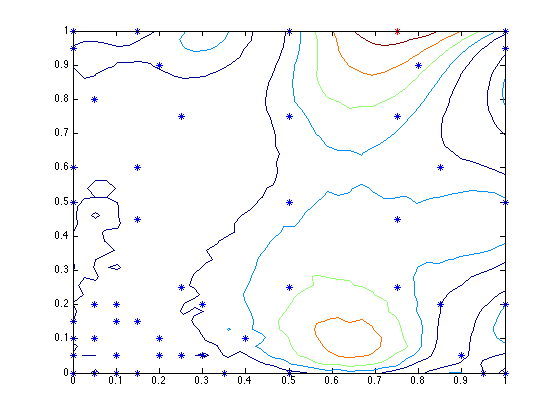
\includegraphics[scale=.27]{centros4_3.png}
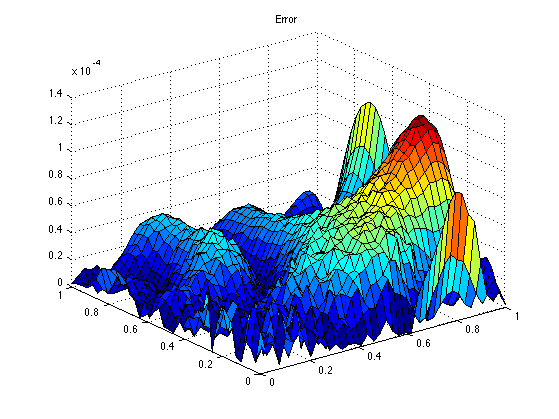
\includegraphics[scale=.27]{error4_3.png}
\caption{Error en la frontera. Parámetro variable}
\end{figure}
\end{document}